\subsubsection{08.12.14}

\begin{enumerate}
	\item Время начала и окончания собрания:
	17:00 - 20:30
	\item Цели собрания:
	\begin{enumerate}
	  \item Выкроить из пластика развертку ковша и склеить его.
	  
	  \item Протестировать то, насколько успешно захват будет закидывать мячи в новый ковш.
	  
    \end{enumerate}
	\item Проделанная работа:
	\begin{enumerate}
	  \item Поскольку листовой ПЭТ нам не удалось приобрести, мы были вынуждены использовать в качестве материала упаковку из ПЭТ-а. В будущем, когда мы сможем купить качественный листовой пластик, мы планируем изготовить ковш из него.
	  
	  \item Развертка ковша была выкроена. Ковш был собран и скреплен изолентой. На следующем занятии мы планируем укрепить швы ковша суперклеем для большей надежности конструкции.
	  
	  \begin{figure}[H]
	  	\begin{minipage}[h]{0.31\linewidth}
	  		\center{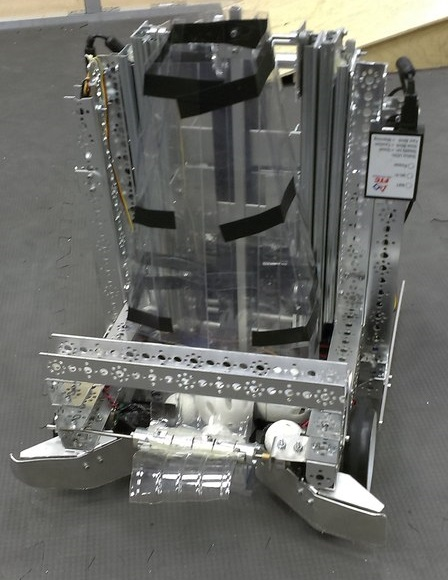
\includegraphics[scale=0.31]{days/08.12.14/images/01}}  
	  	\end{minipage}
	  	\hfill
	  	\begin{minipage}[h]{0.31\linewidth}
	  		\center{
\includegraphics[scale=0.18]{days/08.12.14/images/02}} 
	  	\end{minipage}
	  	\hfill
	  	\begin{minipage}[h]{0.31\linewidth}
	  		\center{
\includegraphics[scale=0.3]{days/08.12.14/images/03}}
	  	\end{minipage}
	  	\vfill
	    \caption{Новый ковш}
	  \end{figure}
      
      \item Были проведены испытания ковша на предмет забора мячей. Когда захват проталкивал мяч к трамплину, закрепленному на ковше, чаще всего он попадал в корзину. Некоторые мячи закатывались вбок и застревали на роботе. Для того, чтобы такого не происходило, по бокам от захвата было решено продлить откосы вверх так, чтобы они не давали мячу уходить в сторону. Некоторые мячи не покидали захват, а проходили в нем полный оборот и выкидывались наружу. Для устранения этой проблемы было решено поставить ограничители, не дающие мячам двигаться вместе с захватом в обратную сторону. После того, как мячи попадали в корзину, они из нее уже не выпадали, поскольку спереди этому препятствовал бортик высотой 7 см, на котором был установлен трамплин.
      
      \item В ходе испытаний было замечено, что, из-за увеличения клиренса передней части робота, маленькие мячи проходят под правым откосом и попадают под днище робота. Чтобы исключить возможность попадания под робота мяча, мы закрепили правый откос на 8 мм ниже. После этого никаких проблем с наездом на мяч не возникало.
      
      \item Поскольку материал, из которого был изготовлен ковш, был очень гибким, во время опрокидывания он прогибался под собственным весом и весом мячей. Чтобы этого не происходило, к задней части ковша был прикреплен тонкий алюминиевый профиль, который поддерживал заднюю стенку корзины. После этого ковш прогибаться перестал.
      
    \end{enumerate}
    
	\item Итоги собрания: 
	\begin{enumerate}
	  \item Ковш собран и установлен на робота.
	  
	  \item Испытания ковша прошли успешно.
	  
	  \item Правый откос закреплен ниже.
	  
    \end{enumerate}
    
	\item Задачи для последующих собраний:
	\begin{enumerate}
	  \item Протестировать механизм опрокидывания ковша на способность перевернуть новый ковш.
	  
	  \item Установить ограничители, не позволяющие мячу попадать мимо ковша.
	  	  
    \end{enumerate}     
\end{enumerate}
\fillpage